\section{Kernels: Neural Path and Neural Tangent}\label{sec:kernels}
In this section, we look at the relationship between the \emph{neural path kernel} (NPK) obtained from the NPFs, and the \emph{neural tangent kernel} (NTK) obtained from the \emph{neural tangent features}. In what follows, let $(x_s,y_s)_{s=1}^n\in\R^{d_{in}}\times\R$ be the dataset. \\
The NPF matrix is given by $\Phi_{\Theta}=(\phi_{x_s,\Theta},s\in[n])\in\R^{P\times n}$. The NPK matrix is then given by $H_{\Theta}=\Phi^\top_{\Theta}\Phi_{\Theta}$. The NPK matrix has a special structure as given in \Cref{lm:npk} below.
\begin{lemma}\label{lm:npk}
Let $p\rsa i$ denote the fact that path $p$ passes through input node $i\in[d_{in}]$, and let $\Lambda_{\Theta}(s,s')\stackrel{def}{=}\sum_{p\rsa i} A_{\Theta}(x_s,p) A_{\Theta}(x_{s'},p)$, $\forall s,s'\in[n]$, any $i\in [d_{in}]$. It follows that $H_{\Theta}= \Sigma\odot\Lambda_{\Theta}$, where $\odot$ stands for the Hadamard product, and $\Sigma \in \R^{n\times n}$ is the input Gram matrix.
\end{lemma}
In the \Cref{lm:npk} above, $\Lambda_{\Theta}\in\R^{n\times n}$ is the correlation matrix of the active sub-networks of different input pairs $s,s'\in[n]$. Note that the definition of $\Lambda$ is not dependent on the choice of input node $i$, because, the terms inside the summation depend only on the path followed from the first layer onwards and excludes the input node.

The \emph{neural tangent feature} (NTF) matrix, denoted by $\Psi_{\Theta}$ is a $d_{net}\times n$ matrix, whose entries are given by $\Psi(\theta,s)=\partial_{\theta} \hat{y}_{\Theta}(x_s),\theta\in\Theta, s\in[n]$\footnote{Here $\partial_{\theta}(\cdot)$ stands for $\frac{\partial (\cdot)}{\partial \theta}$}. The \emph{neural tangent kernel} (NTK) matrix is given by $K_{\Theta}=\Psi_{\Theta}^\top\Psi_{\Theta}$. The NTK is useful in the following two ways:\\
$1.$ Recent works have used the \emph{trajectory} based analysis to show that GD achieves zero training loss in the over-parameterised regime. Suppose we are interested in minimising the squared loss, using GD, and then the trajectory analysis looks at the evolution of the error term $e_t=(\hat{y}_{\Theta_t}(x_s)-y_s,s\in[n])\in\R^n$. The dynamics of the error can given by:
\begin{align}
e_{t+1}=e_t-\alpha_t K_t e_t,
\end{align}
where $\alpha_t>0$ is the stepsize of the GD procedure. Thus, the eigenvalues of $K_t$ play an important role in convergence of GD.\\
$2.$ The NTK matrix has also been used to design pure-kernel based methods \cite{arora2019exact} and provide generalisation bounds \cite{cao2019generalization}.\\
\textbf{NTK in prior works:} Before we connect the NPK and the NTK using the `path-view', we will first look at prior works based on NTK. Prior works have used the following recursive definition or its variants, wherein, for layers $l=1,\ldots, d-1$, we define matrices:
\begin{align}\label{eq:ntkold}
&\tilde{K}^{(1)}(s,s')=\Sigma^{(1)}(s,s')=\Sigma(s,s'), M^{(l)}_{ss'}=\left[\begin{matrix}\Sigma^{(l)}(s,s) & \Sigma^{(l)}(s,s')\\ \Sigma^{(l)}(s',s) & \Sigma^{(l)}(s',s')\end{matrix}\right]\in \R^2,\\
&\Sigma^{(l+1)}(s,s')= 2\cdot\mathbb{E}_{(q,q')\sim N(0,M_{ss'}^{(l)})} \left[\chi(q)\chi(q')\right], \dot{\Sigma}^{(l+1)}(s,s')= 2\cdot\mathbb{E}_{(q,q')\sim N(0,M_{ss'}^{(l)})}\left[\dot{\chi}(q)\dot{\chi}(q')\right],\nn\\
&\tilde{K}^{(l+1)}=\tilde{K}^{(l)}\odot \dot{\Sigma}^{(l+1)}+\Sigma^{(l+1)},\nn
\end{align}
where $s,s'\in[n]$ are two input examples in the dataset, $\Sigma$ is the data Gram matrix, $\dot{\chi}$ stands for the derivative of the activation function with respect to the pre-activation input, $N(0,M)$ stands for the mean-zero Gaussian distribution with co-variance matrix $M$. The final limiting matrix is given by $K^{(d)}=\left(\tilde{K}^{(d)}+\Sigma^{(d)}\right)/2$. Prior works show that at randomised initialisation $\Theta_0$, $K_{\Theta_0}\ra K^{(d)}$ as $w\ra \infty$.\\
\textbf{NTK in `path-view':} Using the `path-view', we obtain a different decomposition for the NTK matrix $K{\Theta}$, and compare our expression to the previously obtained expression in \Cref{eq:ntkold}. To this end, let us by define $d_{net}\times n$ matrices $\Psi^v_t$, and $\Psi^{\phi}_t$, whose entries are given by $\Psi^v_t(\theta,s)=\ip{\phi_{x_s,\Theta},\partial_{\theta}v_{\Theta}}$, and  $\Psi^{\phi}_t(\theta,s)=\ip{\partial_{\theta}\phi_{x_s,\Theta}, v_{\Theta}}$. Now, we have the following NTK decomposition (for a soft-ReLU DNN):
\begin{align}\label{eq:ntknew}
K_{\Theta}=K^v_{\Theta}+K^{\phi}_{\Theta}+(\Psi^v_\Theta)^\top \Psi^{\phi}_{\Theta} +(\Psi^{\phi}_\Theta)^\top \Psi^{v}_{\Theta},\,\text{where},
\end{align}
$K^v_{\Theta}$ is the NTK of path values due to the value gradient, $K^{\phi}_{\Theta}$ is the NTK of the features due to the feature gradient, and $(\Psi^v_\Theta)^\top \Psi^{\phi}_{\Theta} +(\Psi^{\phi}_\Theta)^\top \Psi^{v}_{\Theta}$, is a symmetric matrix which is the cross-term obtained as an interaction of the value and the feature gradients. We now compare expressions in \eqref{eq:ntkold} and \eqref{eq:ntknew},  point out the relationship between NTK and NPK, and discuss the significance of the decomposition in \eqref{eq:ntknew}.\\
\textbf{Comparison of NTK expressions:} The recursive relationship in \eqref{eq:ntkold} is due to the fact that both zeroth-order (forward propagation) and first-order (backward propagation) information use a layer after layer expression for information flow. Also, \eqref{eq:ntkold} derives a limiting matrix ($w\ra\infty$) that occurs at a random $\Theta_0$. On the contrary, \eqref{eq:ntknew} holds for any parameter setting and for finite $w$ and $d$, and further has a term $K^{\phi}_{\Theta}$ that separately models feature learning.\\
 $\bullet$ \textbf{NPK and NTK} $K^v_{\Theta}$, the NTK of path values, describes the dynamics of optimisation due to the value gradient, which, for a given input example, tunes the weights in the active sub-networks. We let $\nabla_{\Theta}v_{\Theta}$ to be the $P\times d_{net}$ matrix consisting of the derivative of the NPVs with respect to the weights of the network, whose entries are given by $\nabla_{\Theta}v_{\Theta}(p,\theta)=\partial_{\theta}v_{\Theta}(p)$. We now expand $K^v_{\Theta}$:
\begin{align}\
K^{v}_{\Theta}=\Phi^\top_{\Theta}(\nabla_{\Theta} v_{\Theta})(\nabla_{\Theta} v_{\Theta})^\top \Phi_{\Theta},
\end{align}
using which and \Cref{lm:nec} we connect the NPK and NTK.
\begin{lemma}\label{lm:nec}
Let $A\in\R^{u\times v}$ and $B\in\R^{w\times u}$, and let $\rho_{\min}(M)$ and $\rho_{\max}(M)$ denote the smallest and the largest eigenvalue of a matrix $M\in\R^{r\times r}$. Then it follows that $\rho_{\min}(A^\top A)\rho_{\max}(B^\top B)\geq \rho_{\min}(A^\top B^\top BA)$.
\end{lemma}
From \Cref{lm:nec}, a necessary condition to ensue that $\rho_{\min}(K^v_{\Theta})$ is bounded away from $0$ is to ensure that $\rho_{\min}(H_{\Theta})$ is bounded away from $0$.\\
\begin{comment}$\bullet$ \textbf{Role of Active Sub-Network:} Input Gram matrix and 
\begin{theorem}[\citet{ando}]\label{th:ando}
For two Hermitian matrices $A\in \C^{d\times d}$ and $B\in \C^{d\times d}$, $\lambda_{\min}(A\odot\B)\geq \lambda_{\min} (AB)$. 
\end{theorem}
\begin{lemma}\label{lm:suf}
For two positive definite symmetric matrices $A$ and $B$, $\lambda_{\min}(AB)\geq \lambda_{\min} (A)\lambda_{\min}(B)$. 
\end{lemma}
From \Cref{lm:suf}, a sufficient condition to ensue that $\rho_{\min}(H_{\Theta})$ is bounded away from zero is to ensure that $\rho_{\min}(\Lambda_{\Theta})$ and $\rho_{\min}(\Sigma)$ bounded away from $0$.\\
\end{comment}
$\bullet$ \textbf{Feature Learning:} $K^{\phi}_{\Theta}$ is the NTK of the features, and describes the dynamics of feature learning due to the flow of the feature gradients, which, for each input example decides, which of the sensitive yet inactive paths should become active, and which of the sensitive yet active paths should become inactive. The NTK of features can be expanded as $K^{\phi}_{\Theta}=\sum_{\theta \in \Theta}\partial_{\theta} \Phi^\top_{\theta}v_{\Theta}v^\top_{\Theta}\partial_{\theta}\Phi_{\Theta}$. The significance here is that $\partial \Phi_{\Theta}$ terms contain, $\partial A_{\Theta}(\cdot,\cdot)$, which in turn contains $\partial G$ terms, which in turn contains $\dot{G}$ term which is the derivative of the gate with respect to its pre-activation input. NTK expression in prior works \eqref{eq:ntkold} only capture the $\chi$ and $\dot{\chi}$ terms. As shown in \Cref{fig:actgate}, only $\dot{G}$ captures the gates that are in the verge of transition (either from $0$ to $1$ or from $1$ to $0$).
%$\bullet$ $(\Psi^v_\Theta)^\top \Psi^{\phi}_{\Theta} +(\Psi^{\phi}_\Theta)^\top \Psi^{v}_{\Theta}$, is a symmetric matrix which is the cross-term obtained as an interaction of the value and the feature gradients.
\FloatBarrier
\begin{figure}[h]
%\begin{minipage}{0.78\columnwidth}
\resizebox{\columnwidth}{!}{
\begin{tabular}{ccc}
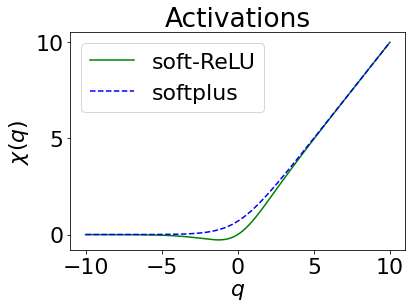
\includegraphics[scale=0.4]{figs/act.png}
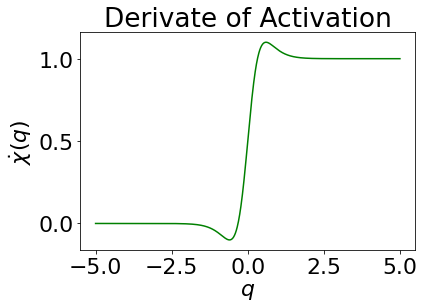
\includegraphics[scale=0.4]{figs/der-act.png}
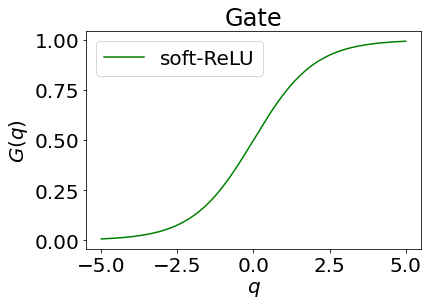
\includegraphics[scale=0.4]{figs/gate.png}
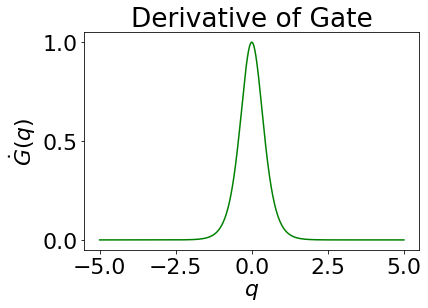
\includegraphics[scale=0.4]{figs/der-gate.png}
%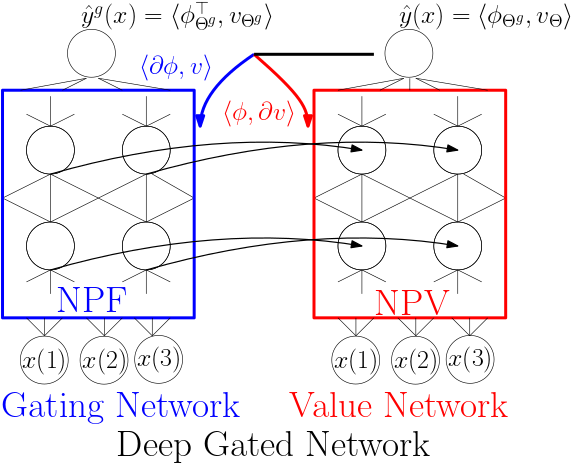
\includegraphics[scale=0.5]{figs/nntwin-blck.png}
%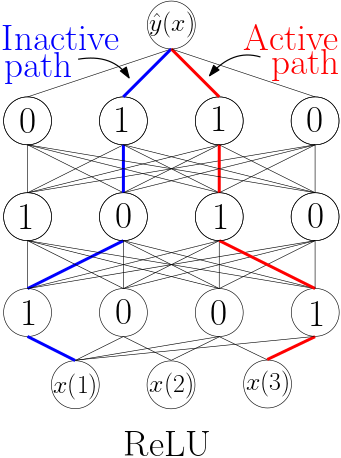
\includegraphics[scale=0.5]{figs/nn.png}
%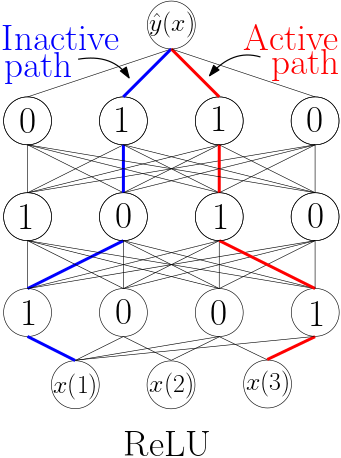
\includegraphics[scale=0.5]{figs/nn.png}
\end{tabular}
}
%\end{minipage}
%\begin{minipage}{0.18\columnwidth}
%\resizebox{\columnwidth}{!}{
%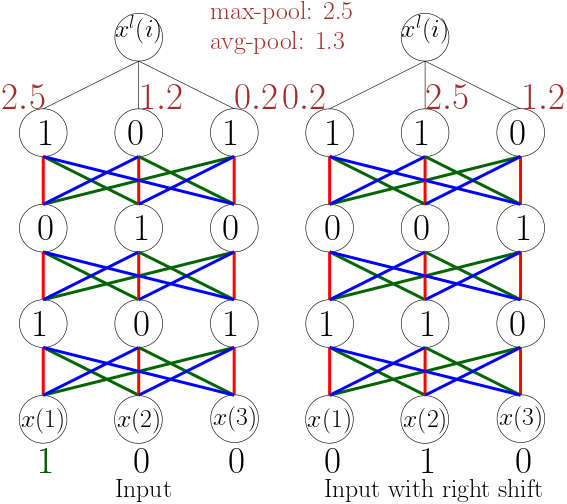
\includegraphics[scale=0.5]{figs/nnconv.png}
%}
%\end{minipage}
\caption{Activations and Gates}
\label{fig:actgate}
\end{figure}

\begin{comment}
\begin{proof}
Matrix $AB$ is similar to the matrix $B^{\frac12}ABB^{-\frac12}$. Thus $\lmin{AB}=\lmin{B^{\frac12}AB^{\frac12}}$.
\begin{align*}
\min_{x: \norm{x}^2=1} x^\top B^{\frac12}AB^{\frac12} x &=  \left(\min_{y: y=B^{\frac12} x, x: \norm{x}^2=1 }y^\top A y \right)\\
%&\geq  \left(\min_{y: \norm{y}^2= \min_{x\in \R^d: \norm{x}^2=1} x^\top B x }y^\top A y \right)\\
&\geq \left(\min_{x: \norm{x}^2=1}x^\top B x \right) \left(\min_{y: \norm{y}^2=1 }y^\top A y \right)
\end{align*}
\end{proof}
\end{comment}